\documentclass[12pt]{article}
\usepackage[utf8]{inputenc}
\pagenumbering{arabic}
\usepackage{graphicx}
\usepackage{amstext}
\usepackage[usenames, dvipsnames]{color}
\usepackage{array}
\usepackage{float}
\usepackage{enumitem}
\usepackage[top=1.5in]{geometry}
\usepackage{subcaption}
\graphicspath{ {images/} }


\begin{document}

\begin{titlepage}
    \begin{center}
    \begin{figure}
        \centering
        
\includegraphics[scale=0.2]{logoPolimi.png}
        \vspace{1.5cm}
    \end{figure}

    \Huge\textbf{Software Engineering 2 Project - Travlendar+}
    \rule{12cm}{0.5pt}
    \Huge\textbf{Design Document - V1}
    \today
    \end{center}
    
    \vspace{3cm}
    
    \begin{flushleft}
        \LARGE\textbf{Authors: }
        \newline\newline
        \Large\texttt{}{Francisco Cristóvão \\ Samsom Tsegay Beyene}
    \end{flushleft}



\end{titlepage}

\newpage
  \tableofcontents
\newpage

\section{Introduction}

\subsection{Purpose}

The main purpose of the Software Design Document (or just Design Document) is to provide a more technical and detailed description about the way Travlendar+ is designed and planned, identifying its main components and the interfaces between them. It also guides the software development team and other interested parties through the architecture of the software project, stating what has to be implemented and how to do it.

\subsection{Scope}
Travlendar+ is a calendar-based application that provides the user a convenient way of organizing his/her daily schedule, maximizing its productiveness and minimizing the worthless time of his/her day. This application was not only thought for the regular businessman/businesswoman, who travel in between meetings the whole day and have no time to spare, but also for the parents with a more regular daily schedule, who just want to get the best out of their time while being able to pick their kids from school and take them to other activities, always being on time.
Of course the system will fully support the features of a regular calendar application (booking of appointments at a specific time and location), but in a "smart" way, being able to detect and warn the user if a new appointment is not feasible because it has a conflict (the start of it doesn't allow the needed travel time after the end of the last appointment) and arranging all of the appointments in the best possible way. The application is meant to be used in the City of Milan, and so it will take advantage of the wide range of travel means and services already existing in the city, from public transports to shared bikes and cars. With the information gathered from those services, it will be able to suggest the best travel mean for the user to move between appointments, based on the available travel time, total cost, current weather and even user preferences.


\subsection{Definitions, Acronyms, Abbreviations}
\subsubsection{Definitions}
\textit{Visitor}: A person who uses Travlendar+ for the first time, and is not yet registered.\\
\textit{User}: A person who uses Travlendar+.\\
\textit{Home Screen}: User interface screen that shows the current appointments.\\
\textit{System}: defines the overall set of software components that implement the required functionality.\\
\textit{Local Time}: time of the system.
\subsubsection{Acronyms}
\textit{API}: Application Programming Interface\\
\textit{DD}: Design Document\\
\textit{ATM: Azienda Trasporti Milanesi}\\
\textit{DD}: Database\\
\textit{SQL}: Structured Query Language\\
\textit{ER}: Entity Relationship Model\\
\textit{MVC}: Model-View-Controller
\textit{SOA}: Service Oriented Architecture
\subsubsection{Abbreviations}


\subsection{Revision History}
Version 1.0: Initial Release

\subsection{Reference Documents}
\begin{itemize}
    \item Assignment document: Mandatory Project Assignments.pdf
    \item Requirements Analysis and Specification Document produced before
\end{itemize}


\subsection{Document Structure}

Other than this introductory chapter, this DD is organized in seven more chapters. Chapter two is meant to \textbf{provide different types of views over the system}:
\begin{itemize}
    \item A high-level overview of how the system is architected.
    \item A description of the main components of the system, their structure and how they interact with each other.
    \item A description of the static deployment view of the system (how the components are deployed in the system's infrastructure). 
    \item A description of the system's behavior and interactions in run-time conditions.
    \item A list of the selected architectural styles and patterns used in the design of the system, as well as the reasons that justify the choice of those patterns.
\end{itemize}

In the third chapter the most \textbf{relevant algorithms} are analyzed and discussed with the appropriate detail and depth, in order to describe the way the system's most critical operations are driven and executed.

The fourth chapter deals with the \textbf{user interface design}. This chapter mainly refers to the mockups provided in the RASD, but it will also include some details on the user interaction with the UI.

The fifth chapter explains how the \textbf{requirements defined in the RASD are fulfilled by the design decisions} that were taken, and how these \textbf{requirements map} to the design elements and decisions defined in the DD.

In the sixth, chapter it is provided a \textbf{implementation, integration and test plan}, defining the order in which the different subcomponents of the system will be implemented, the order in which they will be integrated and how this integration will be tested alongside with the development of the system.

In the seventh chapter the \textbf{effort spent by each of the group member} is described by specifying the number of hours each member of the group worked on the development of this document, and on the final chapter, the tools we used to develop this DD are specified.


\section{Architectural Design}

\subsection{Overview: High-level components and their interaction}

In the following paragraphs it will be presented a general overview of how the system is architected, especially focused on the different logically separated layers.
As described on the RASD, Travlendar+ is supposed to be fully scalable and portable, so a layered architecture is the one that best fits these requirements. Given that the system only provides an Application interface, there's no need for a fourth layer isolating the web server from the application server. 

With this in mind, the system will have a three-layer architecture, organized as shown bellow:
\begin{figure}[H]
    \centering
    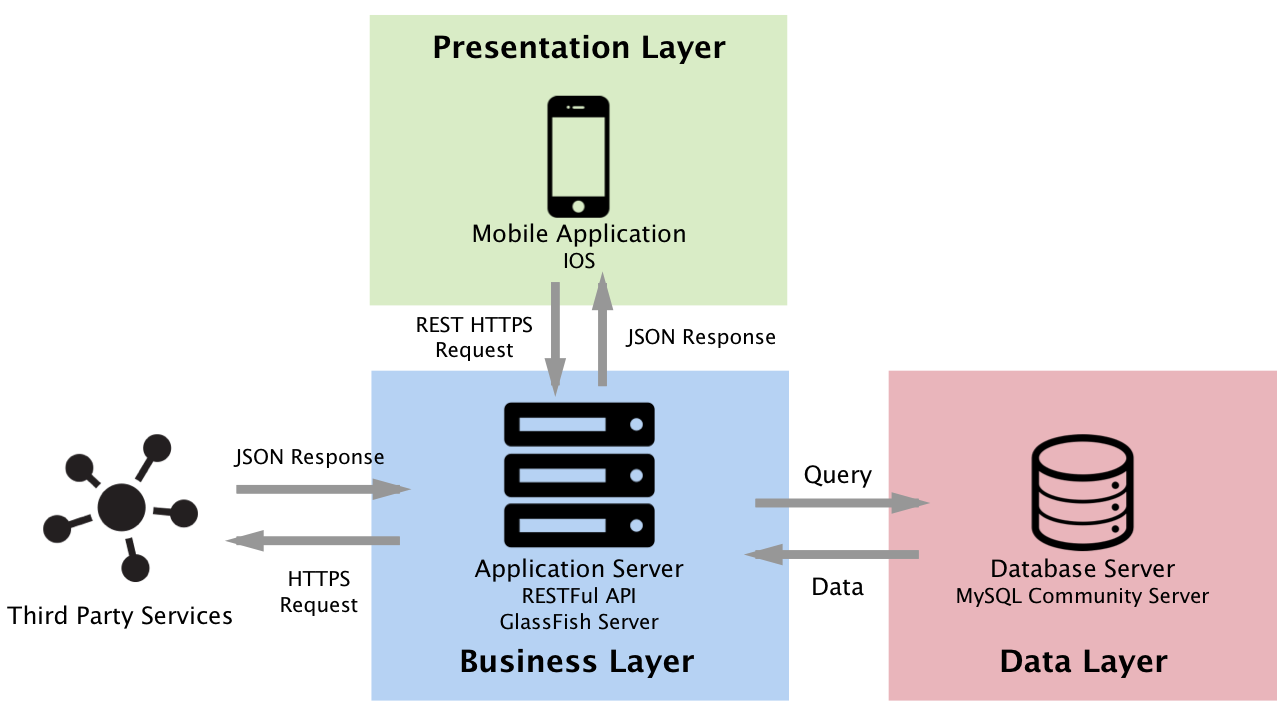
\includegraphics[scale=0.45]{highLevelView.png}
    \caption{High Level View of the system's architecture}
    \label{fig:highLevelView}
\end{figure}
The \textbf{Presentation Layer} is the most external layer of the system, and is responsible for handling all GUI communication and logic. This layer does not handle data or process business rules, but it forwards all the requests to the layers bellow and translates the system operations results of these requests to something that users can understand. It is the only layer of the system that users can access directly and interact with.

The \textbf{Business Layer} implements all core functionality of the system. It's in this layer that the application logic and business rules are implemented, in particular, all the operations related to a user account and the appointment creation and management are performed by components of this layer. Given the importance of this layer (business logic and application server), it should be located in a "demilitarized zone". This layer interacts with the APIs exposed by the Data Layer in order to store and retrieve data. The business layer also depends on some third party systems and the external services they provide (specifically for the implementation of the appointment creation and management and travel mean functionality). These external services are directly invoked by some of the classes of the Business Layer using a public API provided by those.

At last, the \textbf{Data Layer} is the lowest layer of the architecture and includes the data persistence mechanisms responsible for data storage and management (rather than raw DBMS connections). It also provides an API to the Business Layer that exposes methods of managing the stored data without creating dependencies on the data storage mechanisms, promoting the encapsulation of the persistence mechanisms and avoiding data exposition. 

Even though the \textbf{Third Party Services} don't belong to any particular layer, these services are illustrated in the figure above in order to highlight that the interaction with these will happen at the level of the Business Layer.
\subsection{Component View}
The main function of this section is to present a more detailed description of the components that must be developed as part of Travlendar+.

In the following diagram, we can see the component view of the system (the more complex components will be analyzed in further detail).
\begin{figure}[H]
    \centering
    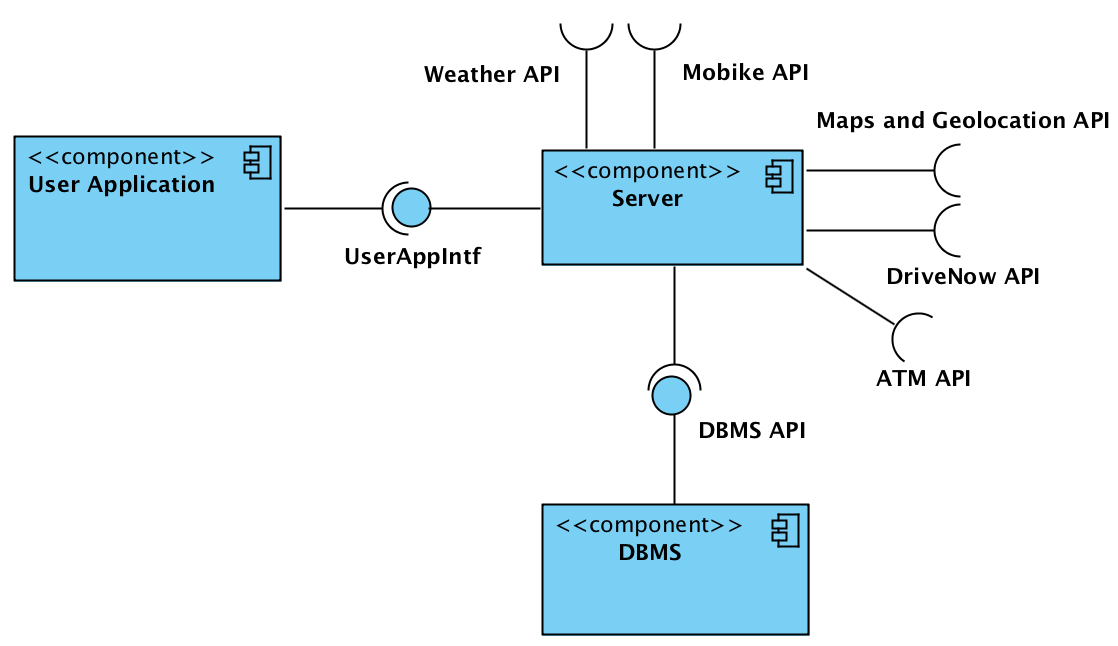
\includegraphics[scale=0.45]{componentView.png}
    \caption{Component Diagram of the system}
    \label{fig:componentView}
\end{figure}
The \textbf{User Application} is the component responsible for providing the user interfaces that allow him to interact with the system and all of its functionality. Since a thin-client is being used to implement a client/server architecture, the bulk of the data processing occurs on the server. Given this, the User Application component will act as a simple "terminal" to send requests to the server, being therefore quite simple and not needed to go into further detail.

The \textbf{Server} is the main component of the system, responsible for the data processing in order to provide all of the system's functionality. Given its complexity, it will be analyzed in further detail later in this section.

The \textbf{Database Management System (DBMS)} is the component responsible for storing and retrieving data in a persistent and reliable way. Instead of implementing this component from scratch, a commercial solution shall be used (MySQL for example).

\subsubsection{Server}
Being the most complex component of the system, it is useful to analyze in detail the Server's constitution.

As mentioned previously, this component is primarily responsible for all operations related to system functionality. More specifically, this component is divided into seven sub-components, each related to a different kind of functionality and operations:
\begin{figure}[H]
    \centering
    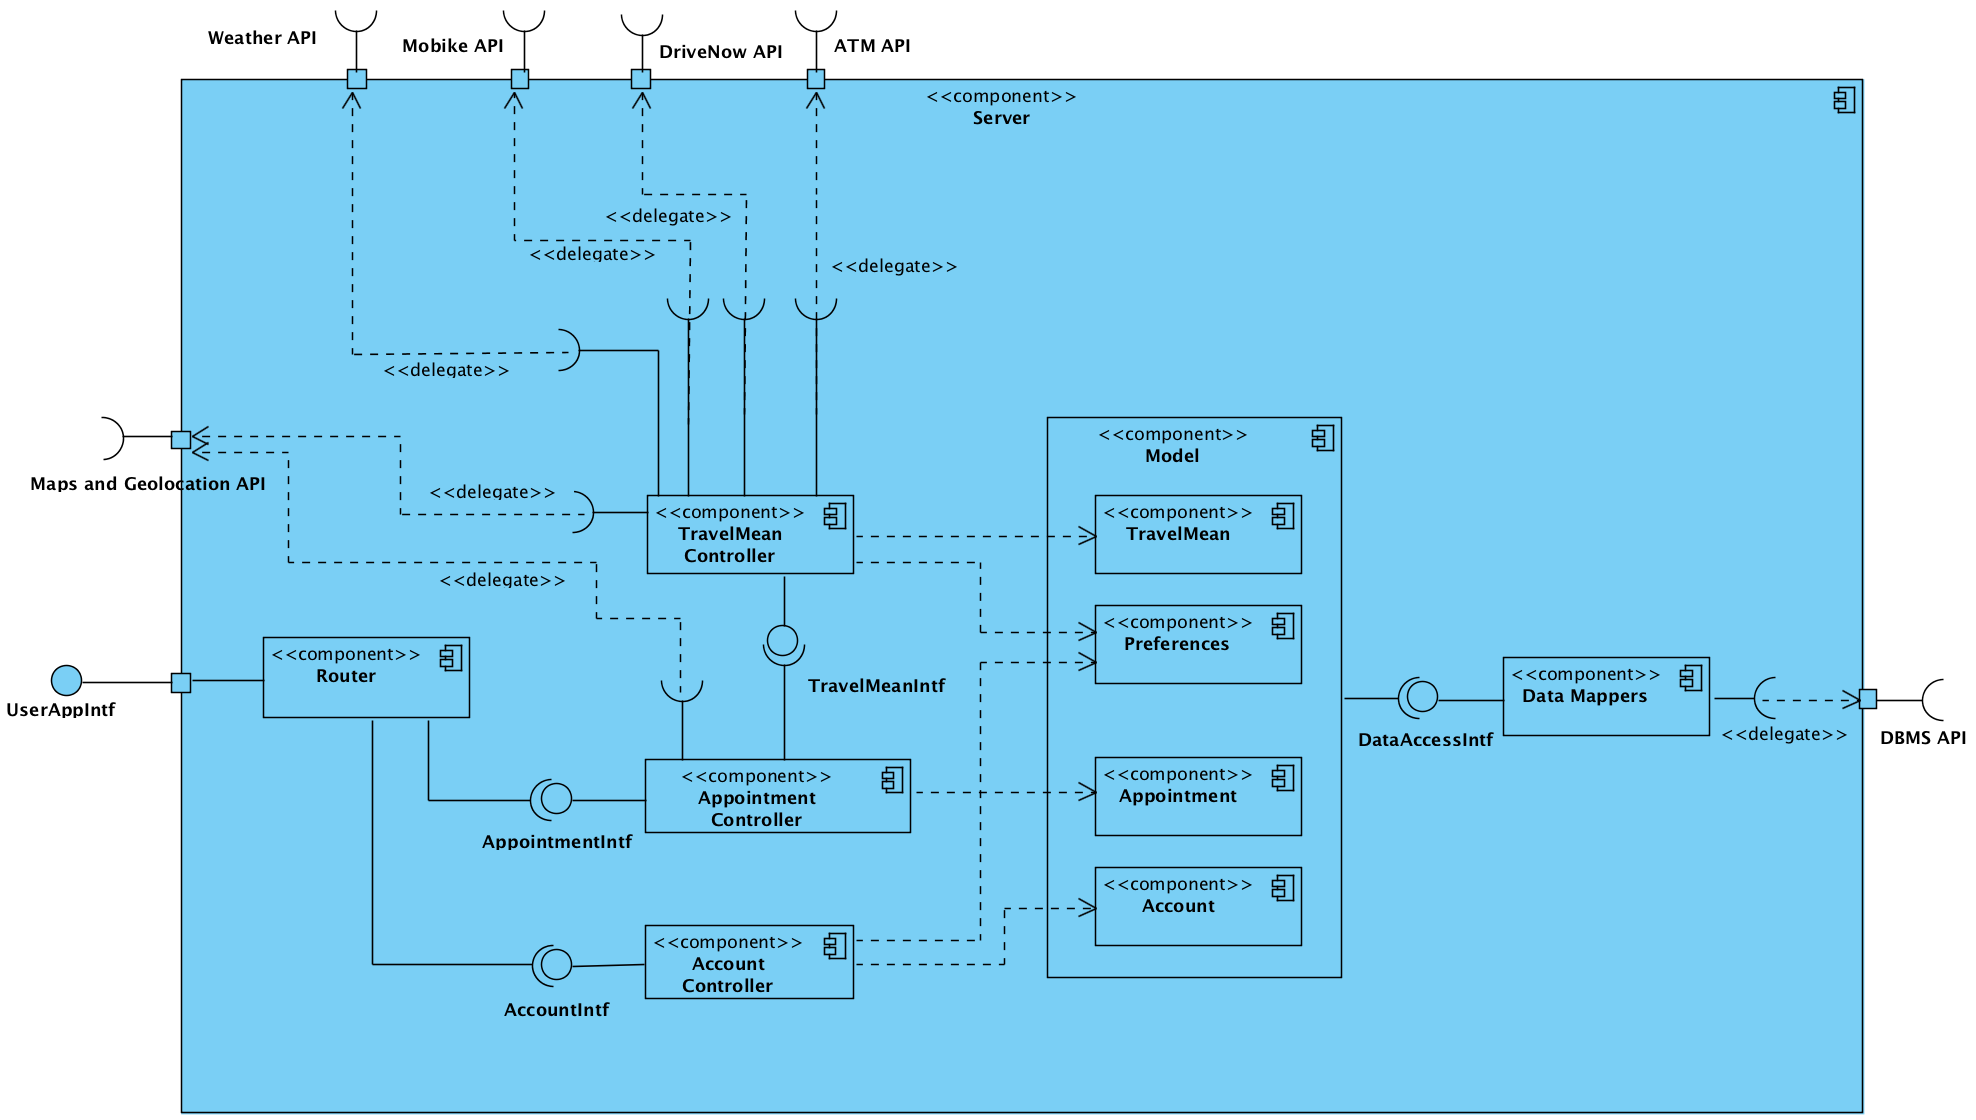
\includegraphics[scale=0.426]{serverComponentView.png}
    \caption{View of Server Component in detail}
    \label{fig:componentView}
\end{figure}
\begin{itemize}
    \item The \textbf{Router} sub-component receives the requests from the User Application and forwards (routes) them to the corresponding controller.
    \item The \textbf{Travel Mean Controller} sub-component performs all the necessary operations to compute the best travel means to get to an appointment, given the schedule at that time. This module is the one with more external interfaces since it needs to gather data from the transport services and weather services in the city of Milan in order to perform its functions.
    \item The \textbf{Location Controller} sub-component implements all methods for updating the location of the user, travel means or appointment, interacting directly with the Maps and Geolocation API.
    \item The \textbf{Appointment Controller} sub-component performs all the necessary operations that allow the user to create, edit and delete an appointment. It is also responsible for all the needed procedures that allow the user to always have the best possible schedule: schedule and arrange the appointments according to the parameters the user defines for each appointment and based on the time the user needs to get from one appointment to another (data computed by the Travel Mean Controller, which explains the dependency from this component). This, allied with the Travel Mean Controller, fulfill all the requirements related to the appointment creation and managing.
    \item The \textbf{Account Controller} sub-component implements all the methods for inserting or updating information about the users. More specifically, it allows the creation of new users (registration of visitors) and login of already existing users. It also performs all the necessary operations to allow the user to edit all of his preferences related to the travel means.
    \item The \textbf{Model} sub-component (and all of its sub-components) manages the behavior and data of the application domain and responds to requests or instructions by the respective controller.
    \item The \textbf{Data Mappers} sub-component is a layer of software which separates the model from the database and acts as a "middle-man" for the interactions between these two.
\end{itemize}


\subsubsection{DBMS}
The following ER provides a graphical representation of the conceptual model of the database.

\subsection{Deployment View}
\subsection{Runtime View}
The following diagrams are intended to describe the interactions between the main system components when performing a sample amount of functionality. These diagrams are still a high-level view of the system, since the function names or even the functions themselves may change during the development process.
\subsubsection{User Login}

\begin{figure}[H]
    \centering
    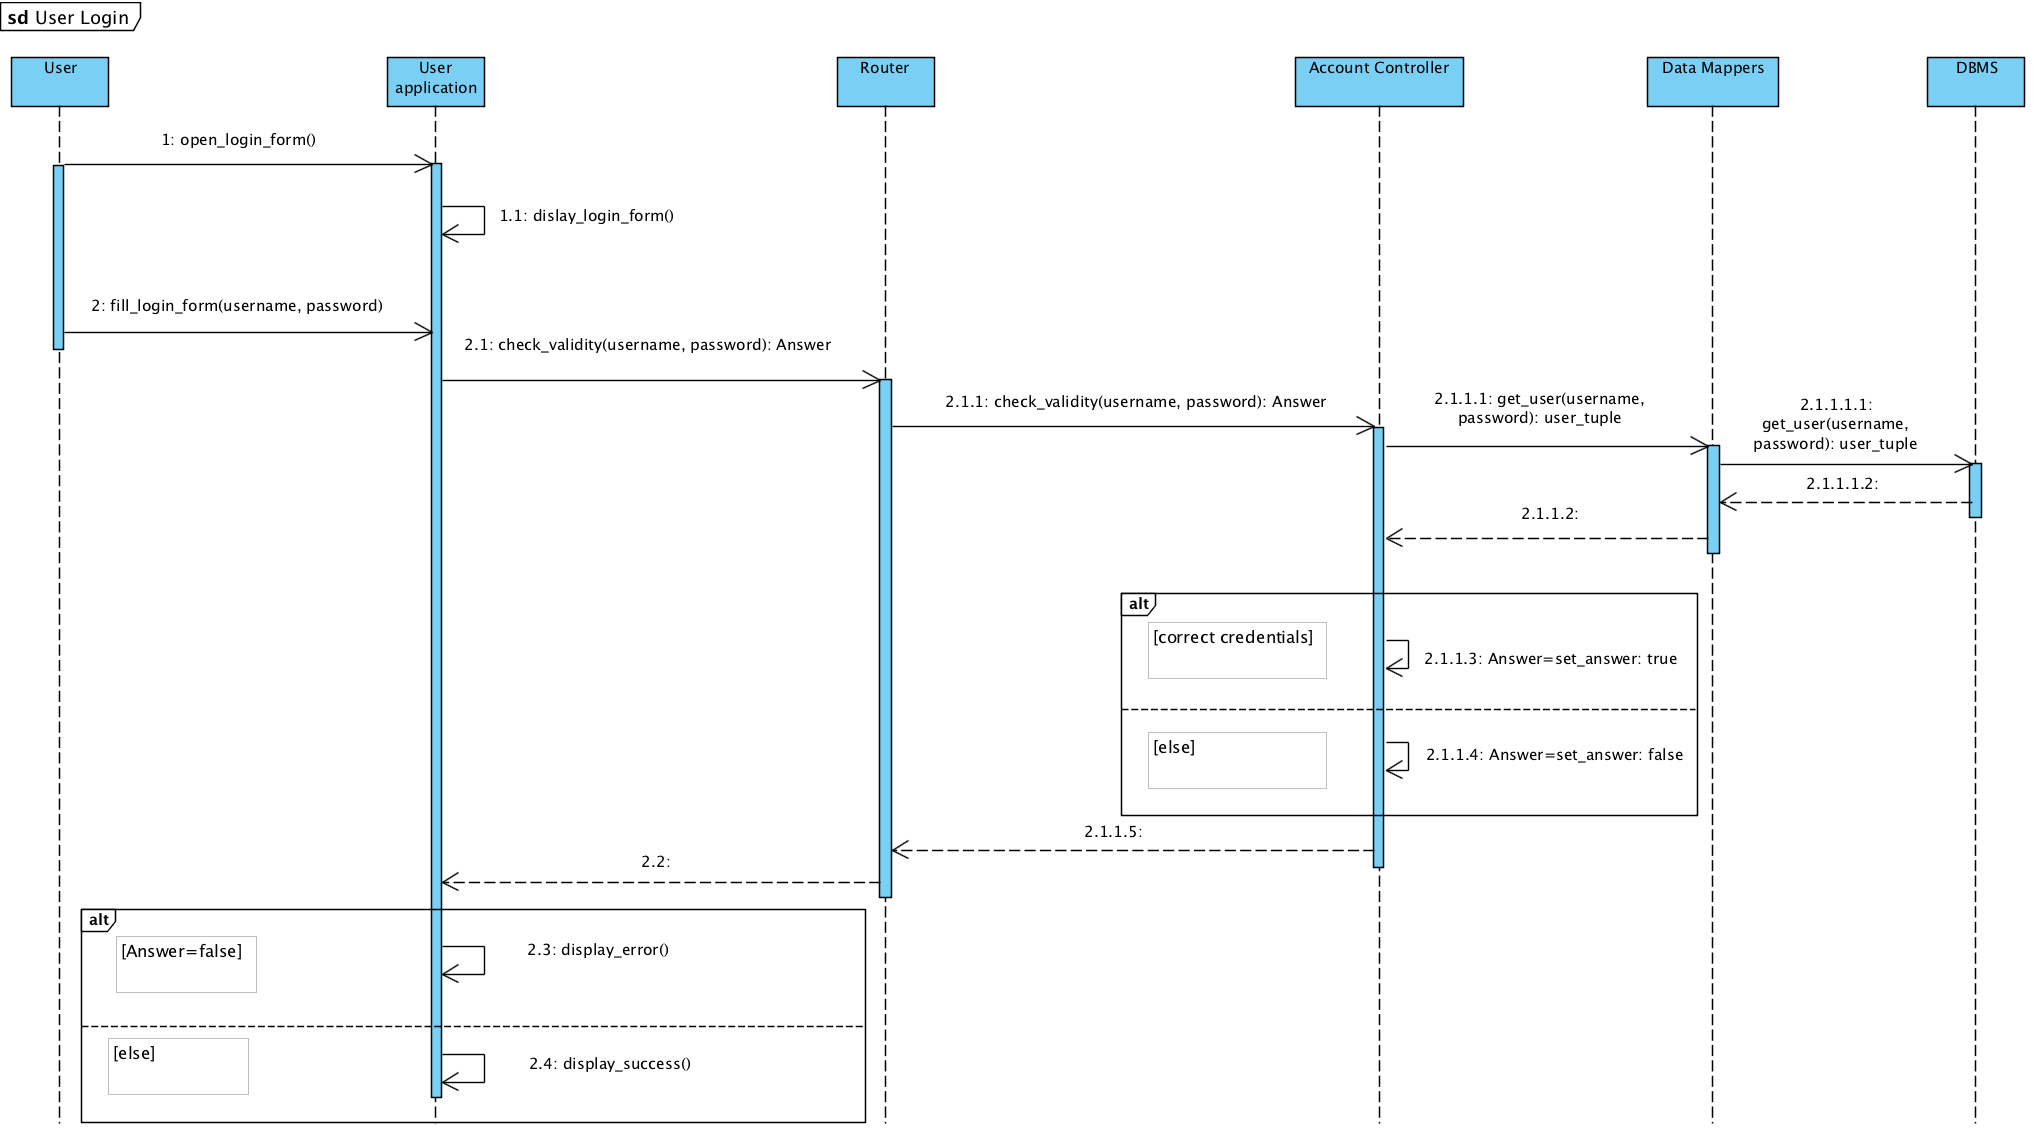
\includegraphics[scale=0.45]{loginRuntimeView.png}
    \caption{User Login}
    \label{fig:loginRuntime}
\end{figure}

\subsection{Component Interfaces}
\subsection{Selected architectural styles and patterns}

\subsubsection{Client/Server Architecture} This architectural style keeps all the logic of the program, which is computationally heavy, on the server side, while the end-users only need to offer a simple amount of presentation functionality. This allows the system to be centralized, improving:
\begin{itemize}
    \item Performance: system's files are only accessed by the server, so they're all in the same place, becoming easier to manage and faster to access
    \item Security: facilitates the implementation of security layers and protocols between the client and the server, setting up access rights to reach the server for example
    \item Scalability: it's easy to change the logic server-side without any implication on the client side
\end{itemize}

\subsubsection{Service Oriented Architecture} This architectural pattern allows the system to be designed as a collection of services that communicate with each other. This way, the external APIs that the system interacts with can be interpreted as a set of these services, which makes them easily implementable (in this case our system is the service consumer, and the APIs are the service providers). It is also possible to see our system as the service provider, first providing an initial set of services and eventually, with the addition of some additional components, increasing the number of services provided.

\subsubsection{Layered Architecture} This architectural pattern promotes a great level of separation of concerns between the various components of the system, given that every component operates at a single logical layer of abstraction. This design choice also simplifies the implementation and testing phase of the system: since the layers are isolated from each other, it is possible to test a specific layer even if the underlying layers aren't implemented, using mocks or stubs to simulate the functionality of those.

\subsubsection{3-Tier Physical Architecture} This architectural style allows the various components of the system on different devices, given the decoupling that exists between the modules. It also allows for any of the three tiers to be upgraded or replaced independently in response to changes in requirements or technology, improving the system's scalability. The system will be composed of 3 tiers: Presentation tier, Business tier (the business logic of the system) and Data tier.

\subsubsection{Model-View-Controller} This architectural pattern divides a given application into 3 interconnected parts, separating the internal representation of information from the way this information is presented to the user. This is one of the most used patterns to promote decoupling between the major components of a system, allowing for efficient code reuse and parallel development.

\subsubsection{Data Mapper} This architectural pattern is a data source architectural pattern. It consists of a layer of software that separates the domain layer objects from the database. Its responsible for transferring data between the two while keeping them isolated from each other and from the mapper itself.
\section{Algorithm Design}

\section{User Interface Design}
\subsection{Mockups}
One of the most important things to take into consideration when designing an information system is the way its functionality is going to be provided to the user. Since the user interacts with our system through a GUI, saying this is the same as saying that this user interface has to be as simple and intuitive to use as possible.

Another thing that was taken into consideration while designing the interfaces was the adaptability of it to the different smartphone screen resolutions and form factors available on the market. To satisfy this requirement, the interface was drawn in a minimalist way, without demanding animations and small details that would make it impossible to use on smaller screens with low resolution.

The mockups of the UI of our system can be found in \textbf{section 3.1.1 of the RASD} and were designed with all this in mind: to be as simple and intuitive to use as possible while providing to the user all of the system's functionality.
\subsection{UX Diagram}
The following UX Diagram provides additional information about the way the user interacts with the system through the mobile application, and have the purpose of complementing the UI mockups provided in the RASD document with a more "dynamic" view over the interface.

\section{Requirements Traceability}

{[G1]} Allow only registered users to access the most relevant functionality of the system.\\
{[G2]} Allow a logged user to create an appointment.\\
{[G3]} Allow a logged user to edit an appointment.\\
{[G4]} Allow a logged user to delete an appointment.\\
{[G5]} Allow a logged user to have his schedule planned in the best possible way.\\
{[G6]} Allow a logged user to define preferences related to travel means.

\section{Implementation, Integration and Test Plan}

\section{Effort Spent}

\begin{center}
\begin{tabular}{ |p{0.25\textwidth}|p{0.4\textwidth}|p{0.25\textwidth}| } 
 \hline
 \textbf{DATE} & \textbf{TASK} & \textbf{HOURS} \\ 
  \hline
 08/11/2017 &  Scope, Purpose and Document Structure & 1 \\ 
  \hline
 09/11/2017 & Overview and Architectural Styles and Patterns & 3 \\
  \hline
  10/11/2017 & High Level Components description and Database Component View & 4 \\ 
  \hline
  11/11/2017 & Component View and Architectural Styles and Patterns & 3 \\ 
  \hline
  12/11/2017 & Component View and Architectural Styles and Patterns & 1,5 \\ 
  \hline
  13/11/2017 & Component View and Deployment View & 4 \\ 
  \hline
  14/11/2017 & Component View, Architectural Styles and Patterns and Component Interface & 3 \\ 
  \hline
  17/10/2017 & Use Case Description and User Interface & 4 \\ 
  \hline
  18/10/2017 & Runtime View and User Interface (UX Diagram) & 3,5 \\
  \hline
  \textbf{TOTAL} & \multicolumn{2}{c|}{27} \\ 
  \hline
\end{tabular}
\end{center}

\section{References}
https://www.safaribooksonline.com/library/view/software-architecture-patterns/9781491971437/ch01.html

https://martinfowler.com/eaaCatalog/index.html

Patterns of Enterprise Application Architecture, Martin Fowler

\end{document}